

\tikzset{every picture/.style={line width=0.75pt}} %set default line width to 0.75pt        

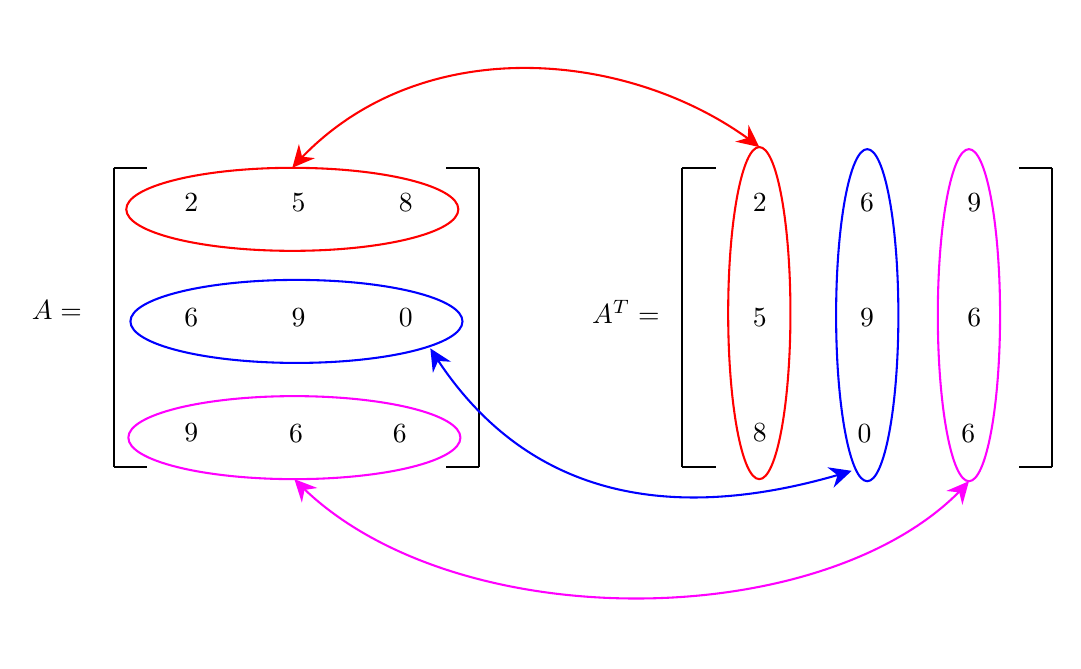
\begin{tikzpicture}[x=0.75pt,y=0.75pt,yscale=-1,xscale=1]
%uncomment if require: \path (0,300); %set diagram left start at 0, and has height of 300

%Straight Lines [id:da2213819570252611] 
\draw    (93.89,70) -- (93.89,214) ;
%Straight Lines [id:da29721507169372896] 
\draw    (93.89,70) -- (110,70) ;
%Straight Lines [id:da35934426602025504] 
\draw    (93.89,214) -- (110,214) ;

%Straight Lines [id:da6023748561134159] 
\draw    (270,214) -- (270,70) ;
%Straight Lines [id:da4805786206905196] 
\draw    (270,214) -- (253.89,214) ;
%Straight Lines [id:da5967411370774598] 
\draw    (270,70) -- (253.89,70) ;

%Straight Lines [id:da9049186085059904] 
\draw    (367.78,70) -- (367.78,214) ;
%Straight Lines [id:da6931297695132848] 
\draw    (367.78,70) -- (383.89,70) ;
%Straight Lines [id:da7325439366388315] 
\draw    (367.78,214) -- (383.89,214) ;

%Straight Lines [id:da9297150199392166] 
\draw    (546.11,214) -- (546.11,70) ;
%Straight Lines [id:da17597738471086588] 
\draw    (546.11,214) -- (530,214) ;
%Straight Lines [id:da9212767075909833] 
\draw    (546.11,70) -- (530,70) ;

%Shape: Ellipse [id:dp6011237777220346] 
\draw  [color={rgb, 255:red, 255; green, 0; blue, 0 }  ,draw opacity=1 ] (100,90) .. controls (100,78.95) and (135.82,70) .. (180,70) .. controls (224.18,70) and (260,78.95) .. (260,90) .. controls (260,101.05) and (224.18,110) .. (180,110) .. controls (135.82,110) and (100,101.05) .. (100,90) -- cycle ;
%Shape: Ellipse [id:dp9649907352391565] 
\draw  [color={rgb, 255:red, 255; green, 0; blue, 0 }  ,draw opacity=1 ] (405,60) .. controls (413.28,60) and (420,95.82) .. (420,140) .. controls (420,184.18) and (413.28,220) .. (405,220) .. controls (396.72,220) and (390,184.18) .. (390,140) .. controls (390,95.82) and (396.72,60) .. (405,60) -- cycle ;
%Shape: Ellipse [id:dp49968264093049886] 
\draw  [color={rgb, 255:red, 0; green, 0; blue, 255 }  ,draw opacity=1 ] (102,144) .. controls (102,132.95) and (137.82,124) .. (182,124) .. controls (226.18,124) and (262,132.95) .. (262,144) .. controls (262,155.05) and (226.18,164) .. (182,164) .. controls (137.82,164) and (102,155.05) .. (102,144) -- cycle ;
%Shape: Ellipse [id:dp12864677020337312] 
\draw  [color={rgb, 255:red, 255; green, 0; blue, 255 }  ,draw opacity=1 ] (101,200) .. controls (101,188.95) and (136.82,180) .. (181,180) .. controls (225.18,180) and (261,188.95) .. (261,200) .. controls (261,211.05) and (225.18,220) .. (181,220) .. controls (136.82,220) and (101,211.05) .. (101,200) -- cycle ;
%Shape: Ellipse [id:dp02487303364640492] 
\draw  [color={rgb, 255:red, 0; green, 0; blue, 255 }  ,draw opacity=1 ] (457,61) .. controls (465.28,61) and (472,96.82) .. (472,141) .. controls (472,185.18) and (465.28,221) .. (457,221) .. controls (448.72,221) and (442,185.18) .. (442,141) .. controls (442,96.82) and (448.72,61) .. (457,61) -- cycle ;
%Shape: Ellipse [id:dp312374845137267] 
\draw  [color={rgb, 255:red, 255; green, 0; blue, 255 }  ,draw opacity=1 ] (506,61) .. controls (514.28,61) and (521,96.82) .. (521,141) .. controls (521,185.18) and (514.28,221) .. (506,221) .. controls (497.72,221) and (491,185.18) .. (491,141) .. controls (491,96.82) and (497.72,61) .. (506,61) -- cycle ;
%Curve Lines [id:da9481816921410489] 
\draw [color={rgb, 255:red, 255; green, 0; blue, 0 }  ,draw opacity=1 ]   (182.71,66.99) .. controls (242.07,2.98) and (344.32,13.49) .. (403.23,58.62) ;
\draw [shift={(405,60)}, rotate = 218.31] [fill={rgb, 255:red, 255; green, 0; blue, 0 }  ,fill opacity=1 ][line width=0.08]  [draw opacity=0] (10.72,-5.15) -- (0,0) -- (10.72,5.15) -- (7.12,0) -- cycle    ;
\draw [shift={(180,70)}, rotate = 311.19] [fill={rgb, 255:red, 255; green, 0; blue, 0 }  ,fill opacity=1 ][line width=0.08]  [draw opacity=0] (10.72,-5.15) -- (0,0) -- (10.72,5.15) -- (7.12,0) -- cycle    ;
%Curve Lines [id:da7276678073856719] 
\draw [color={rgb, 255:red, 0; green, 0; blue, 255 }  ,draw opacity=1 ]   (248.45,160.11) .. controls (291.17,226.83) and (359.47,243.25) .. (446.85,216.81) ;
\draw [shift={(449.5,216)}, rotate = 522.72] [fill={rgb, 255:red, 0; green, 0; blue, 255 }  ,fill opacity=1 ][line width=0.08]  [draw opacity=0] (10.72,-5.15) -- (0,0) -- (10.72,5.15) -- (7.12,0) -- cycle    ;
\draw [shift={(246.5,157)}, rotate = 58.44] [fill={rgb, 255:red, 0; green, 0; blue, 255 }  ,fill opacity=1 ][line width=0.08]  [draw opacity=0] (10.72,-5.15) -- (0,0) -- (10.72,5.15) -- (7.12,0) -- cycle    ;
%Curve Lines [id:da16259241119309786] 
\draw [color={rgb, 255:red, 255; green, 0; blue, 255 }  ,draw opacity=1 ]   (183.24,222.32) .. controls (257.48,297.18) and (438.48,294.33) .. (504.05,223.18) ;
\draw [shift={(506,221)}, rotate = 491.08] [fill={rgb, 255:red, 255; green, 0; blue, 255 }  ,fill opacity=1 ][line width=0.08]  [draw opacity=0] (10.72,-5.15) -- (0,0) -- (10.72,5.15) -- (7.12,0) -- cycle    ;
\draw [shift={(181,220)}, rotate = 46.7] [fill={rgb, 255:red, 255; green, 0; blue, 255 }  ,fill opacity=1 ][line width=0.08]  [draw opacity=0] (10.72,-5.15) -- (0,0) -- (10.72,5.15) -- (7.12,0) -- cycle    ;

% Text Node
\draw (126.54,80.95) node [anchor=north west][inner sep=0.75pt]    {$2$};
% Text Node
\draw (178.2,80.95) node [anchor=north west][inner sep=0.75pt]    {$5$};
% Text Node
\draw (229.86,80.95) node [anchor=north west][inner sep=0.75pt]    {$8$};
% Text Node
\draw (126.54,136.4) node [anchor=north west][inner sep=0.75pt]    {$6$};
% Text Node
\draw (178.2,136.4) node [anchor=north west][inner sep=0.75pt]    {$9$};
% Text Node
\draw (229.86,136.4) node [anchor=north west][inner sep=0.75pt]    {$0$};
% Text Node
\draw (126.54,191.85) node [anchor=north west][inner sep=0.75pt]    {$9$};
% Text Node
\draw (177,192.4) node [anchor=north west][inner sep=0.75pt]    {$6$};
% Text Node
\draw (227,192.4) node [anchor=north west][inner sep=0.75pt]    {$6$};
% Text Node
\draw (53,132.4) node [anchor=north west][inner sep=0.75pt]    {$A=$};
% Text Node
\draw (400.43,80.95) node [anchor=north west][inner sep=0.75pt]    {$2$};
% Text Node
\draw (452.09,80.95) node [anchor=north west][inner sep=0.75pt]    {$6$};
% Text Node
\draw (503.75,80.95) node [anchor=north west][inner sep=0.75pt]    {$9$};
% Text Node
\draw (400.43,136.4) node [anchor=north west][inner sep=0.75pt]    {$5$};
% Text Node
\draw (452.09,136.4) node [anchor=north west][inner sep=0.75pt]    {$9$};
% Text Node
\draw (503.75,136.4) node [anchor=north west][inner sep=0.75pt]    {$6$};
% Text Node
\draw (400.43,191.85) node [anchor=north west][inner sep=0.75pt]    {$8$};
% Text Node
\draw (450.89,192.4) node [anchor=north west][inner sep=0.75pt]    {$0$};
% Text Node
\draw (500.89,192.4) node [anchor=north west][inner sep=0.75pt]    {$6$};
% Text Node
\draw (323,132.4) node [anchor=north west][inner sep=0.75pt]    {$A^{T}=$};


\end{tikzpicture}